\section{Bias variance tradeoff}

The bias-variance framework provides a structured approach to evaluating model performance. 
In this framework, we represent the data as a combination of a deterministic component and noise with zero mean and variance $\sigma^2$:
\[t=f(\mathbf{x})+\varepsilon\]

\paragraph*{Known process}
When the underlying process $f(\mathbf{x})$ generating the data is known, the correct model $y(\mathbf{x})$ for the given process can be determined using Population Risk Minimization:
\[y^\ast(\mathbf{x})=\argmin_{y\in\mathcal{H}}\mathbb{E}_{t,x}[(t-y(\mathbf{x}))^2]=\int\Pr(\mathbf{x})(f(\mathbf{x})-y(\mathbf{x}))^2\,d\mathbf{x}\]

\paragraph*{Unknown process}
When the underlying process is unknown, we use Empirical Risk Minimization:
\[\hat{y}(\mathbf{x})=\argmin_{y\in\mathcal{H}}\dfrac{1}{N}\sum_{n=1}^n(t_n-y(x_n))^2\]
Here, the random variable $\hat{y}$ depends on the dataset. 

The expected squared error can then be decomposed as follows:
\[\underbrace{\mathbb{E}_{\mathcal{D},t}\left[ {\left( t-\hat{y}(\mathbf{x}) \right)}^2 \right]}_{\text{error}} = \underbrace{\sigma^2}_{\text{irreducible error}}  +  \underbrace{\text{Var}_{\mathcal{D}}\left[\hat{y}(\mathbf{x}) \right]}_{\text{variance}}  +  \underbrace{\mathbb{E}_{\mathcal{D}}{\left[f(\mathbf{x}) -\hat{y}(\mathbf{x}) \right]}^2}_{\text{squared bias}}\]
In this decomposition:
\begin{itemize}
    \item \textit{Expected error}: averaged over the training dataset $\mathcal{D}$ and the target $t$.
    \item \textit{Irreducible error}: unaffected by model choice or the number of samples.
    \item \textit{Variance}: measures variability between models trained on different datasets, reducing as model complexity decreases or as the sample size grows. 
        High variance leads to overfitting.
    \item \textit{Squared bias}: measures the deviation between the true function and the expected learned function, depending on the hypothesis space $\mathcal{H}$. 
        Bias generally decreases with model complexity. 
        High bias results in underfitting.
\end{itemize}
\begin{figure}[H]
    \centering
    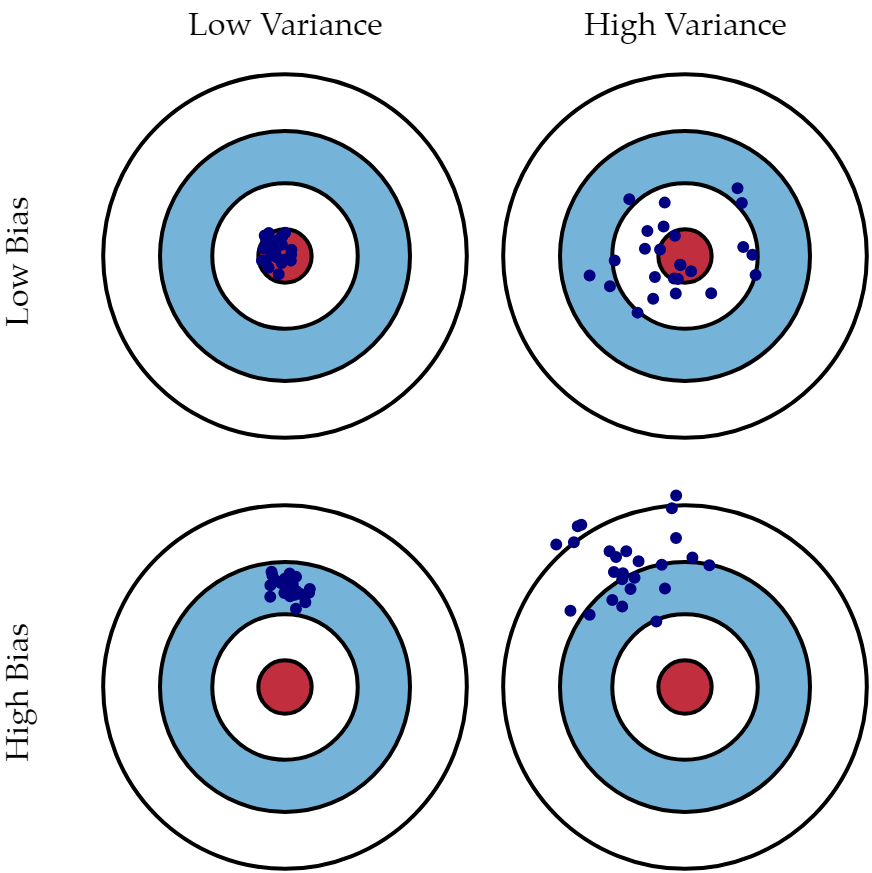
\includegraphics[width=0.5\linewidth]{images/bvf.png}
    \caption{Bias-variance framework}
\end{figure}
The bias-variance decomposition shows why regularization helps reduce error on unseen data. 
Lasso regression tends to outperform Ridge regression when only a few features contribute to the output.

\subsection{Training error}
Given a dataset $\mathcal{D}=\left\{ \mathbf{x}_i,t_i \right\}$ with $i=1,\ldots, N$, a model is chosen based on the computed loss $\mathcal{L}$ over $\mathcal{D}$. 
For regression, the loss function is:
\[L_{train}=\dfrac{1}{N}\sum_{n=1}^N{\left(t_n-y(\mathbf{x}_n)\right)}^2\]
The training error decreases as model complexity increases.
However, training error does not provide an accurate estimate of the error on new data, known as the prediction error. 
For regression, the prediction error is represented by:
\[\mathcal{L}_{true}=\iint{\left( t-y(\mathbf{x})\right)}^2\Pr(\mathbf{x},t)\,d\mathbf{x}dt \]
Modeling the joint probability distribution $\Pr(\textbf{x}, t)$ is often infeasible.

In practice, data is typically split into a training set and a test set. 
Model parameters are optimized using the training set, and prediction error is estimated using the test set.
As the sample size grows, training and test errors converge. 
Examining train and test errors helps identify issues:
\begin{itemize}
    \item \textit{High bias}: when both training and test errors are high and close to each other.
    \item \textit{High variance}: when training error is low, but test error gradually increases to match it.
\end{itemize}
\begin{figure}[H]
    \centering
    \begin{subfigure}{0.32\textwidth}
        \centering
        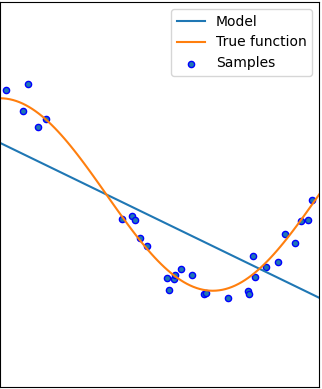
\includegraphics[width=0.75\linewidth]{images/hb.png} 
        \caption{High bias}
    \end{subfigure}
    \begin{subfigure}{0.32\textwidth}
        \centering
        
\includegraphics[width=0.75\linewidth]{images/b.png} 
        \caption{Balanced}
    \end{subfigure}
    \begin{subfigure}{0.32\textwidth}
        \centering
        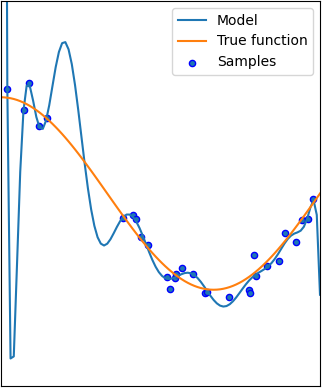
\includegraphics[width=0.75\linewidth]{images/hv.png} 
        \caption{High variance}
    \end{subfigure}
    \caption{Bias-variance balancing}
\end{figure}
When data is limited, test error may appear minimal, leading to under- or over-estimation of the prediction error. 
Using test error for model selection can result in overfitting to the test set. 
An unbiased estimate of prediction error is only achievable if the test set remains separate from training and model selection processes.